\documentclass{article}
\usepackage[utf8]{inputenc}
\usepackage[toc,page]{appendix}
\usepackage[backend=biber,style=ieee,dashed=false,sorting=ynt]{biblatex}
\usepackage{tabularx}
\usepackage{diagbox}
\addbibresource{sources.bib}
\usepackage{todonotes}
\usepackage{verbatim}
\usepackage{hyperref}
\usepackage{graphicx}
\usepackage{titlesec}

\setcounter{secnumdepth}{4}

\titleformat{\paragraph}
{\normalfont\normalsize\bfseries}{\theparagraph}{1em}{}
\titlespacing*{\paragraph}
{0pt}{3.25ex plus 1ex minus .2ex}{1.5ex plus .2ex}

\title{Group E Report \\
    \Large DevOps, Software Evolution and Software Maintenance \\
    Course Code: BSDSESM1KU}
\author{Julian Brandt - jubr@itu.dk,\\
        Jakub Sowa - jsow@itu.dk,\\ 
        Nicolai Pallund - npal@itu.dk,\\ 
        Mads Ørnfeldt Wolf Jespersen - oeje@itu.dk,\\ 
        Osman Abdinasir Hassan - osha@itu.dk}
\date{June 2022}

\begin{document}

\maketitle

\newpage
\tableofcontents
\newpage

\section{Introduction}
This report describes the process of developing and maintaining an application "MiniTwit", which is a simple Twitter clone. The project was made as a part of the Spring 2022 course DevOps, Software Evolution and Software Maintenance. The finished application can be viewed on the website \href{http://shittytwitter.ml}{http://shittytwitter.ml}, and the code for the application can be viewed in our GitHub repository: \cite{repository}.

\section{Process}
\subsection{Team work}
When the project first started, we quickly decided on a set of rules to help us throughout the project. Such rules were for example: we would always create new branches for features, never push directly to the master branch on GitHub, and use Discord for both communication, as well as a place to share app secrets between group members. To discourage rule breaking, if someone were to break a rule, they would owe beers or something similar for a final celebration once the project was over.

The team would always meet up on campus on Tuesdays, which was the designated work day for the DevOps course. Here we would discuss the previous weeks work, what everyone was working on currently, and what people planned on doing until next week. We often ate lunch together on this day as well, and sometimes played ping pong after class to help us get to know each other, and to help us wind down after a day of work.

\subsection{Version Control}
Git was picked as the version control system for this project, and was used through GitHub. Everyone in the group was familiar with Git and GitHub already, so we could get quickly started with the project. By using GitHub, we were also able to use GitHub Actions in our workflow, which will be explained in further detail in section \ref{ci_cd_hub}.

\subsection{Work practices}
The team has mainly been working in smaller groups of 1-2 people on each task throughout the project. As the group consisted of 5 people in total, it did not make sense to involve the entire group in each task, as it would simply not be efficient use of development time.

\subsubsection{Work division}
To keep track of tasks to be done, we used GitHub Projects, which is a Kanban board directly attached to GitHub. It allowed us to quickly create tasks from GitHub Issues, as well as assign developers and branches to said tasks. This was under-utilized throughout the project, but was picked up again near the hand-in date, where it proved to be very helpful to create a final to-do list. Outside of the Kanban board, we also reminded each other of tasks to be done through other communication channels, such as Discord or in person.

\subsubsection{Branch strategy}
When a new task was being worked on, people involved were to create a new branch on the GitHub repository, with a fitting name of the feature, which was to be merged into a central development branch at a later point. Once the task was done, at least one person outside of the task had to review the pull request. Afterwards, the new feature was discussed in the group, either online or in person, ensuring everyone was caught up to speed. When the central development branch had had a reasonable amount of changes, it would be merged into the master branch, and then deployed automatically.

\section{Technologies}
This section will briefly describe the entire technology stack, and our reasoning for each technology, sometimes comparing them to competitors.

\subsection{Application Framework}
We chose ASP.Net as our framework for the web application for multiple reasons: Support, maturity and familiarity. ASP.Net also provides built-in support for many things that we will need, including but not limited to: session management, object-relational mapping, model-view-controller design pattern, security and server-side rendering.

Appendix A (\ref{languagechoice}) is a more in-depth discussion of different languages and frameworks, and Appendix C (\ref{scriptinglanguages}) is a description of the scripting languages we used in CI/CD.

\begin{description}
\item [Support] In 2021, the most popular non-JavaScript web framework was ASP.NET Core
\cite{so_market_share}). As ASP.NET Core is currently one of the largest web frameworks, there is a large amount of support available, as the community is very active and it is usually easier to troubleshoot problems, as someone likely has had the same issues before.
\item [Maturity] ASP.Net has been in development for 20 years, and has become solid software that will reliably fit into most tech stacks.
\item [Familiarity] A less technical reason for choosing ASP.Net is that the group was already familiar with it, which would likely reduce development time
\end{description}

\subsection{Object-Relational Mapping Framework}
To manage data between application and database, we use the Object-relational mapping library Entity Framework. This particular framework was chosen partly because we were familiar with it, but also because of the following points: \\

\noindent Entity Framework provides a lot of useful tools and features for web applications, such as: 
\begin{description}
\item [lazy loading] which improves performance, postponing the execution of a query until it is actually needed
\item [query translation/inspection] which allows for checking how the actual queries performed on the database look like, and enables us to tweak them to improve the performance
\item [changes tracking] which makes deploying the database schema changes easier, since it takes a single command to generate a migration based on the current state and a new database schema definition, and seldom have to make decisions on how something should be migrated.
\end{description}

\subsection{Database Management System}
Since we are only storing data about users and their tweets, a standard DBMS like PostgreSQL, MySQL or MS SQL Server is sufficient, with none having a major benefit over another. We ended up going with Postgres, because of our cloud provider and our familiarity with PSQL. During our consideration we compared the scalability of various solutions - even NoSQL options with their horizontal scaling - but we did not foresee that Postgres would cause us any issues.

\subsubsection{Hosting on Digital Ocean}
Our choice of DBMS has also been heavily affected by the fact that Digital Ocean (our chosen cloud provider) offers hosting a managed database, which automatically logs all database transactions and backs up our data independently of our application. While hosting the database and application separately increases response time per query, it simplifies difficult problems with data-migration during redeployment.

\subsection{Provisioning Tool}
For this project we have opted for using Vagrant as a virtual machine provisioning tool. It is \textit{lightweight} in the sense that you only need a "vagrantfile" to provision a new cloud hosted virtual machine, and run an initialization script on it - essentially deploying the service from nothing by running a single file. This was initially a very attractive choice, as this file can simply be shared over GitHub, and any team member or deployment service would be able to provision and start the application. While a Docker image of the web server might have taken more initial set-up of containerizing the application, had we been able, we would probably have switched to Docker, because of maturity issues with Vagrant. Vagrant is not as common as Docker, and thus not available out-of-the-box for services like GitHub Actions, and with limited support/issues with Digital Ocean.



\subsection{CI/CD Hub} \label{ci_cd_hub}
The need for a good CI/CD pipeline required us to find a tool, that could easily integrate into our workflow. The simplest solution, was to use the built-in solution provided by GitHub: GitHub Actions, which allows one to create pipelines by using \textit{.yaml} files, and then to inspect their results on GitHub. One can argue that GitHub Actions is a poor choice, since we would rely even more on GitHub being online, and if GitHub goes down, we would lose access to all the pipelines. For that reason, we were considering using Travis CI, however we did not want to pay out of pocket for a tool for the project, so we settled on GitHub Actions, and accepted the risk of the service being offline.
Even when using other CI/CD solutions, they would have to be integrated into our repository, in order to allow for functionalities like testing on pushes to a branch. GitHub would have to be online for that to work anyway.

\subsubsection{Automatic releases}
As part of the project we had to do regular releases of our code. GitHub Actions can automatically release when new code is pushed to master, which we have set up, such that the latest release always has the newest version without us having to write anything.



\subsection{Cloud Provider} \label{digitalocean}
For this project, we picked Digital Ocean as the cloud provider to host both the application and other necessary infrastructure, as well as the PostgreSQL database. 

In the group, we have members who have either used Amazon Web Services, Azure or Digital Ocean before. These three were therefore the main competitors in our optics.

Amazon Web Services and Azure provides a lot of different services that Digital Ocean does not. In return, Digital Ocean is (in our eyes) much more user friendly for non-experts, where the AWS dashboard and Azure portal can be a mouthful. Digital Ocean has an easy to understand interface with one-click deployments, as well as an intuitive API which can be invoked with a token. \\

\noindent In the end it came down to the fact that we each had \$100 of free credit for Digital Ocean's services.

\subsection{Load Balancing and Scaling} \label{dockerswarm}
Towards the latter half of the project we began moving towards using Docker Swarm, rather than the singular Digital Ocean droplet.

There were a couple of reasons that made Docker Swarm an attractive approach for orchestrating the services in our system. The tool allowed us to change our deployment strategy from a blue-green strategy to a rolling update strategy instead, allowing the singular instances within the swarm to be updated one at a time, which should allow for faster updating once scaled horizontally. It also has a built in load balancer, allowing for much easier distribution between worker nodes. Because of these functionalities, Docker Swarm provides an approach that is more favorable if the application should be scaled to match a growing number of user requests.

One of the main reasons for why we choose Docker Swarm over other orchestration tools, is the relative ease of use and implementation into our existing setup.

\section{Software Maintenance}

\subsection{Continuous Integration and Continuous Deployment}
During the project, we set up a pipeline for continuous integration and deployment. The pipeline begins with someone creating a pull-request to the dev branch from a feature branch. The code from the feature branch is automatically built and tested with \texttt{dotnet test} when pushed, so we know it works and is ready to be merged. Once the pull request is reviewed and merged, the dev branch can be merged into master, which starts our deployment pipeline. The pipeline works in the following steps:
\begin{enumerate}
    \item SSH into the deployer-machine.
    \item Load environment variables into the deployer (tokens, ssh keys, connection strings, etc.).
    \item Clone repository onto deployer.
    \item Create environment for the web server.
    \item Run \texttt{vagrant up} on deployer to provision the web server VM.
    \item Run scripts to replace old production server with the new one, if the new deployment was successful.
\end{enumerate}

\subsubsection{SSH into the deployer}
The deployer is a machine hosted separately from GitHub for two reasons. It decreases our dependence on GitHub, letting us deploy even if GitHub is down. It also gives more freedom to configure our deployer-machine, since GitHub Actions does not have an out-of-the-box image with Vagrant on Linux, which we would then have to configure ourselves anyways.

\subsubsection{Load environment variables}
Since we do not want to store secrets in our public repository, we use GitHub Actions to store our secrets, and load them into environment variables during deployment. This also lets us switch the target machine-name that Vagrant uses by exporting a new environment variable, which simplifies swapping between the old production server and the new temp server.

\subsubsection{Clone repository onto deployer-machine}
The deployer clones the repo such that it can transfer the application to the web server. 


\subsubsection{Create environment for web server}
The database and logging connection strings are loaded as environment variables. The deployer creates a script \texttt{env.sh}, which loads the connection string into the environment of the web server. The script is then used as part of the Vagrant provisioning.

\subsubsection{Run \texttt{vagrant up} on deployer}
The web server is provisioned and the program is started on port 80.

\subsubsection{Run scripts to replace the old production server}
Now that the server should be running, we need to make sure that it is actually alive, after which we can replace the old production server through a blue-green strategy. We have three scripts that run after each other:
\begin{enumerate}
    \item \texttt{MinitwitAlive.py} repeatedly sends a request for the front page to the newly opened web server. If it responds with status code \texttt{200}, we assume that the server works.
    \item \texttt{reassign\_floating\_ip.py} moves a static IP from the old production server to the newly provisioned server. If this script succeeds, the old production server is shut down, having seamlessly replaced the production server without downtime.
    \item \texttt{rename\_droplet.py} renames the new server from \textit{temp} to \textit{prod}.
\end{enumerate}

\subsubsection{New version is deployed}
When all these steps have completed without errors, we have successfully deployed the newest version of the application. If any of these steps fail, the new deployment is rolled back with a failure on the GitHub Actions page.

\subsection{Monitoring}
\subsubsection{Stack}
To monitor the application, we used a basic Prometheus-Grafana setup consisting of:
\begin{itemize}
    \item Calls to Prometheus metrics library within source code 
    \item Prometheus instance that aggregates the metrics
    \item Grafana instance for displaying the data
\end{itemize}

\subsubsection{Provisioning}
Both Grafana and Prometheus are provisioned using configurations stored inside the "monitoring" folder in our repository.

Furthermore, we have dockerized both setups and created a Vagrant file, allowing us to start the monitoring service with a single command.
\paragraph{Problems}
While provisioning of the Prometheus instance worked flawlessly, we encountered some issues with Grafana. Namely, the provisioning files for database as a data source were not working correctly, so we had to insert some details manually each time.

It was also very difficult to provision an automatic alert/notification system, so we decided to do that manually, since provisioning of this server happens infrequently.

\subsubsection{Visualization}
\paragraph{Idea}
Grafana was used to help visualize metrics, to gain insight into the usage of the application.

Since everything in our app heavily relies on database queries, we decided to time each of them to see how fast they are. 

To understand the average user better and to see how much data we actually have, we added database queries as another data source.

Finally, in order to see how well the system performs, and how many resources it uses, we added some metrics that display those parameters. In case the system went down, Grafana would alert us through a specified channel on Discord.

\paragraph{Results}
Thanks to the visualization, we managed to fix some issues regarding database queries. We could also see usage patterns and act accordingly in case we would need to. At one point in the project, we also got a notification from the outage-alerter during development, which we quickly fixed.

\subsection{Logging}
\subsubsection{Setup}
Our logging setup consists of 4 components:
\begin{itemize}
    \item Serilog - utility for Asp.NET for logging the events, with a target set as an Elasticsearch instance
    \item Elasticsearch - for searching and aggregating the logs
    \item Kibana - for visualizing the logs 
    \item Nginx - reverse proxy for restricting access to other components
\end{itemize}
Much like in the monitoring case, the whole stack was dockerized, and a Vagrant file was created for deployment purposes. The machine used for serving the logs had to be a bit bigger in terms of RAM (4gb), otherwise Elasticsearch and Kibana would not work.
It occurred to us later in the project, that the server's 80GB disk filled up rather quickly, as we had not set a "time to live" on the logs. Ideally, this would be set to two weeks or so. In the end, this meant that we were not able to index the logs, due to lack of space.

\subsubsection{Idea}
We wanted to have the ability to inspect queries that were being made to the database. This, with the addition of out-of-the-box logging allowed us to have a full overview of what the application was doing.

\subsubsection{Result}
As part of project we introduced an intentional bug somewhere in the application, and had another part of the group attempt to identify it with only the logs we collect.
The results of this bug-hunt can be seen in \cite{bugs}.

\subsection{Risk Analysis}
\subsubsection{Risk Matrix}
In this section we present the results of our internal security audit, for a more in-depth description of the items in the matrix please see appendix \ref{securityanalysis}.

\noindent Below is a table showcasing the likelihood of identified risks and their impact if they were to be exploited.

\begin{tabularx}{1\textwidth} { 
  | >{\raggedright\arraybackslash}X 
  | >{\raggedright\arraybackslash}X 
  | >{\raggedright\arraybackslash}X 
  | >{\raggedright\arraybackslash}X 
  | >{\raggedright\arraybackslash}X 
  | >{\raggedright\arraybackslash}X | }
 \hline
 \diagbox[width=1\textwidth/8+2\tabcolsep\relax, height=1.3cm]{Likelihood }{Impact} & very low & low & medium & high & critical \\
 \hline
 very low & & & DDOS & Open ports & SQL injection \\[8ex]
 \hline
 low & & & & XSS &\\[8ex]
 \hline
 medium & & & & & Unauthor-ized access \\[8ex]
 \hline
 high & Knowledge of stack & & & &\\[8ex]
 \hline
 very high & & & Big messages & &\\[8ex]
\hline
\end{tabularx}


\subsubsection{Solutions/mitigations}
Based on the risk analysis and the problems we found, we came up with solutions to mitigate some of the issues.
\begin{description}
    \item [Big messages.] Sending long messages to saturate the network connection can be mitigated heavily by imposing character limits on the length of messages. \textbf{This was implemented by the team.}
    \item [Open ports.] There is a multitude of port scanning tools available that would allow the team to ensure no port is left open. \textbf{This was implemented by the team.}
    \item [Unauthorized access.] The likelihood of leaking secrets is reduced by us enforcing required reviews on pull requests to the repository, making uploading keys less likely. Likewise the developers should ensure that no authentication information is shared through insecure methods. \textbf{This was exercised by the team.}
    \item [DDOS.] There are a few defense measures one can employ to reduce the impact of DDOS attacks, such as rate limiting, detecting bot patterns and blacklisting bad actors. Some of these measures are hard to build, and is therefore usually outsourced to companies like CloudFlare.
\end{description}

\section{Stack Diagram}
We have created a diagram to give an overview of our infrastructure and how every service interacts. It shows how the system uses four virtual machines and one managed database to run everything.
\begin{figure}[h]
    \centering
    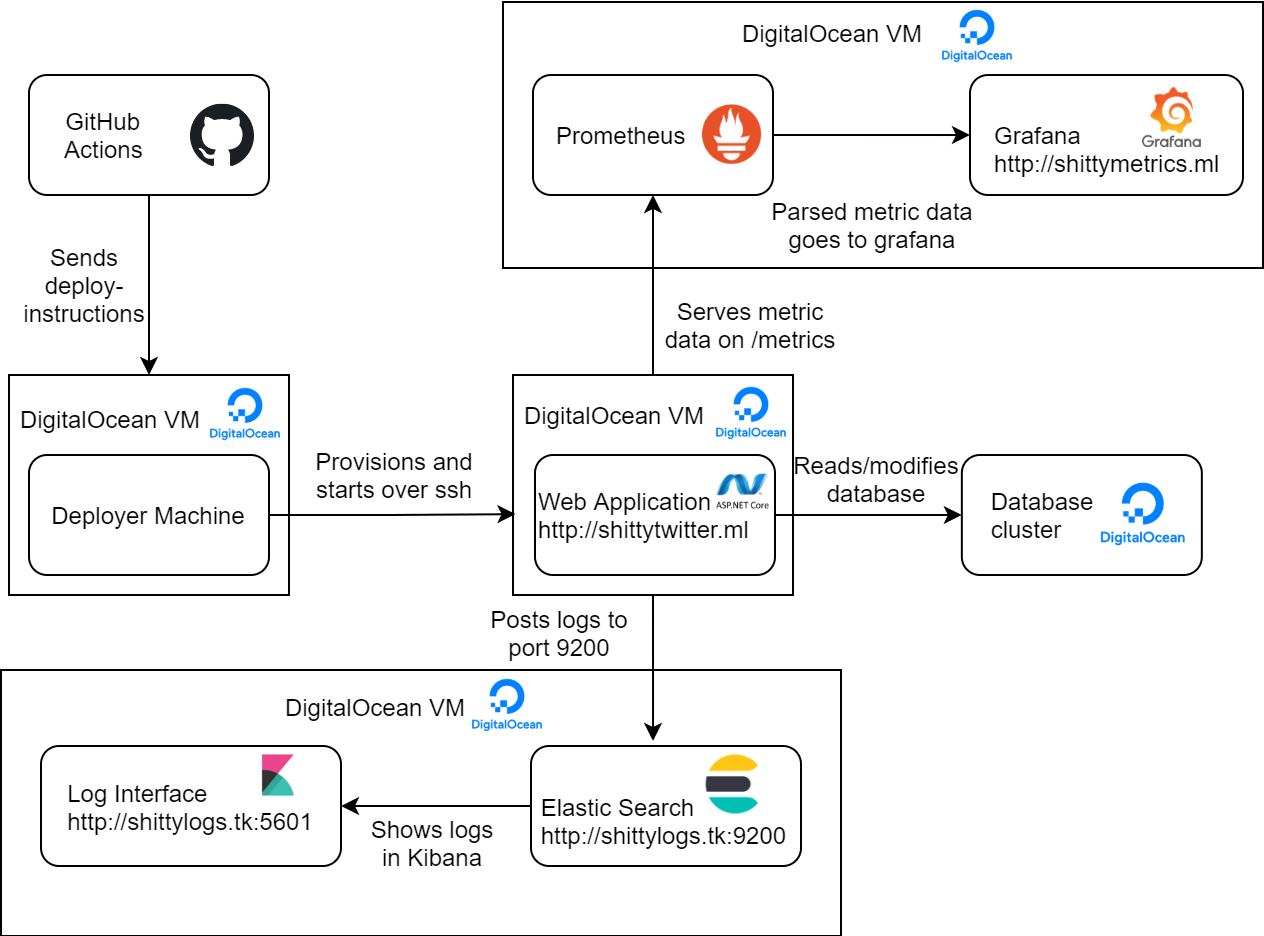
\includegraphics[width=1\linewidth]{images/technologies.png}
    \caption{Complete diagram of all services}
    \label{fig:technology_diagram}
\end{figure}

\section{Status on Static Analysis}
The static analysis tools we have used are SonarQube (through SonarCloud), Code Climate, Better Code Hub, Snyk, CodeQL and ActionLint. Badges showing the status of all the run tools can be viewed at the top of the \texttt{readme.md} file in the GitHub repository \cite{repository}.
\begin{description}
\item [Sonar Cloud:] The output of our latest run on Sonar Cloud can be seen here in \cite{sonarcloud}, and shows that we get a score of 'A' on every mark. We have some code smells which relate to null references in the code when we fetch from the database.
\item [Code Climate:] Code Climate gives us a good maintainability score, with an 'A' in technical debt. It can be found in \cite{codeclimate}
\item [Better Code Hub:] We could not get better code hub to exclude parts of our repository (like the old python version of MiniTwit), which results in it giving us a lower score, with many errors. Because of this, we have put less emphasis on the results from Better Code Hub, in comparison to the other tools.
\item [Snyk:] Snyk was used to analyse packages and their vulnerabilities. As of writing this report, there are no found vulnerabilities in the MiniTwit project, but throughout the project we used snyk to fix vulnerabilities in a dependency called "Gravatar Helper" and outdated system packages.
\item [CodeQL:] CodeQL notified us of hard coded user credentials which were for testing, and some false positive security flaws, due to how the system is built. 
\item [ActionLint:] We used ActionLint to verify that our scripts on GitHub Actions were not malformed, and thus would not run. As of writing this report they are all correctly formed.
\end{description}

\subsection{Code coverage}
Using \texttt{dotnet test} to capture code coverage in our application. At first glance we get a \textit{fairly bad} score of 13\%. This is because it includes a bunch of automatically generated files, such as database migrations, as well as our frontend cshtml, which we agreed not to test. When we narrow our coverage to just the controllers, as well as what we call "Repository files" (files that access the entities, such that the controllers do not access the database directly), we improve to 47.6\%. While it is still a relatively low score, we do not test our controllers since they only call the "Repository" files, which are fully tested. Because of this, we believe we have acceptable code coverage, while we could still add tests in controllers.


\subsection{License}

We have run the ScanCode toolkit to check the licenses of the application, and everything uses the MIT license, apart from the Open Iconic font, which has its own license added in the repository. By the results of this \cite{scancode}, we have decided to use the MIT license for the application.


\section{Perspective}
\subsection{Structuring of infrastructure}
We decided early that separating major parts of our infrastructure into separate machines/images/etc. would be a good way to structure the project. As the project progressed, we came to appreciate this separation, as it made each piece easier to manage and easy to swap out.

A concrete example would be our separation of the main application and the database. This separation made deployment easier than trying to move the data from one VM to another without losing it.

\subsection{Concurrent deployment caused outage}
We used GitHub Actions to deploy our application, unaware of the fact that GitHub Actions defaults to running actions concurrently, instead of queuing them if multiple are triggered. This caused one of our deployment-scripts to fail in such a way that both the new and old production VMs were shut down simultaneously, leaving us without a production server. This was caused by us merging multiple feature branches into the main branch at the same time, and was before we had set up alerts, so the outage lasted for about 30 minutes before we realized the site had gone offline.

The learning experience we acquired from this issue, is that we have to think of our infrastructure just like our code, with critical sections and all the other considerations that comes with concurrent access to shared resources.\\

We fixed the issue by introducing a flag to make that specific action queue its runs, instead of doing them concurrently:\\
\href{https://github.com/ChadIImus/Devoops/commit/d84b7f3386f1c9106bc173767507488977856268}{Fix on github.com}


\subsection{Handling secrets}

During the project work, we had one case of secrets being leaked:
\href{https://github.com/ChadIImus/Devoops/commit/8f034df248d53f19b084fa88ce6c546c87714843}{Fixed leak}

Secrets were kept on the deployer VM, which used them to deploy the application, and the rest were kept on separate platforms such as Discord and GitHub Actions Secrets. This kept it out of anyone else's hands, but ideally we would have set up some machine/key-vault that kept all secrets stored in one place and when needed we fetch them programmatically with individual secrets for each developer. There are two reasons for this. The separate platforms required developers to manually fetch zip files with keys, or copy paste keys individually, so the process was not very streamlined. Security was also at risk, since the secrets were shared over Discord, which meant that Discord kept logs of our messages.

\subsection{Quality of tools}
We learned that investing time in finding the best tool or workflow is just as important as working with said tool. Our experience with GitHub Actions and Vagrant showcases this well. When we started using GitHub Actions, we found some working examples and went from there. At some point, we encountered an error, and were then left to keep pushing changes to the action to see if the problem was fixed. 

We later discovered that there are tools for running actions locally, which allow for faster iteration time, and much better debugging. \\

\noindent Our experience with Vagrant as a provisioning tool was also not the best. It is quite slow - even when we did not use it with GitHub Actions. 

We found it very difficult to use SSH keys with Vagrant. Vagrant kept trying to use local keychains or would load the SSH keys in with wrong formatting, and it kept breaking when running the vagrantfile on different members' computers. When we later used Digital Ocean's API and Docker for creating dockerized hosts, we discovered that it was much faster and gave us more freedom to choose how we wanted to interact with the VMs, after they were provisioned. The reduced iteration time would have made configuring our supporting infrastructure more productive, as each attempt with Docker would be several minutes quicker than Vagrant. 



\section{Bibliography}
\printbibliography[title={Bibliography}]


\section{Appendix}
\subsection{Appendix A - Choice of the main language (C\#)} \label{languagechoice}
\subsubsection{Our measures}
One of the hardest decisions to begin this project, was to pick the programming language that would work the best. A couple of things we had to take into account were performance, implementation time, difficulty of usage, support, stability, maturity, feature mapping and many more. 
\subsubsection{Python}
Initially, we considered working with Python and Django, since that would make refactoring the initial application much easier while also making the development time extremely fast due to the structure of the language, and the group's experience with Python. After careful consideration, we decided to give up on this idea, since Python does not support explicit typing, which might result in some unnoticed runtime errors. The other factor that influenced our decision was the "running" speed. Python is slower than other considered languages, and it does not support multithreading natively, so we would need to use special libraries, which would result in a higher memory overhead and would detract from the ease of use which python in known for.
\subsubsection{Functional Languages}
We considered functional languages as well, however we gave up on the idea rather fast, because most of our team is not as experienced in functional paradigm, meaning the development of the application would be more difficult. A major downside was also our lack of knowledge or experience of the frameworks present in these ecosystems.
\subsubsection{C\#}
After some consultation, we decided to go for a language that is object-oriented, since we all know this paradigm quite well. We also wanted to pick a language that has a fast execution time. Based on these criteria, we decided to settle for C\#, since it is relatively fast compared to Python for instance. It also has a lot of support in terms of online documentation and libraries, and is really mature in terms of feature it supports. C\# is also the choice for many in the corporate world, which also was a considerable benefit.
This choice is not necessarily the definitive best choice, as every programming language has their respective pros and cons, but we decided that C\# was most fitting choice for our group, and allowed us to expand our knowledge in other areas, such as Razor Pages as well as the new technologies.

\subsection{Appendix B - SQL Vs NoSQL} \label{sqlvsnosql}
\subsubsection{SQL vs NoSQL} 
In recent times, there is a huge debate over whether to use SQL or NoSQL databases with web applications. There are a lot of advantages to using either structure. NoSQL databases are often used when working with big datasets that need to scale well. NoSQL offers great support for unstructured data that can be accessed quickly. On the other hand, the standard SQL keeps the database in a consistent state, and provides a high amount of integrity, which we find more important than scalability in this project. Another important factor is that the previous database from the MiniTwit Python was also a SQL one, which would makes the transition to another SQL-based solution much easier.

\subsection{Appendix C - Scripting languages} \label{scriptinglanguages}
To allow for easier development, we have decided to automate some tasks with popular scripting languages, so that we would not have to click so much, in turn reducing our workload.

\subsubsection{Shell}
We have been using shell, as it is the standard on all ubuntu systems, which make most of the currently running servers. Furthermore, all of the most important CLI commands are also ported into Powershell, so it is quite easy to to run those scripts on windows. The shell scripts are extremely useful, when we have to do system wide operations such as installing a program or setting up a development environment. They also come in handy when we need to use some CLI tools such as the ones for building our web application or running the tests.

\subsubsection{Python}
Even though we did not choose Python as our main development language, it is still very valuable. We used it for scripting as these relatively lightweight scripts are well suited to pythons strengths, such as dynamic typing and speed of development. 

\subsection{Appendix D - Security analysis} \label{securityanalysis}
\subsection{Risk Identification}
\subsubsection{Assets}
The application consists of multiple services and tools that could all potentially be vulnerable to an attack. These are:
\begin{itemize}
    \item Web application and stack
    \item Digital Ocean droplets
    \item ELK logging chain
    \item Metrics service (Grafana)
    \item GitHub source control (public repository)
\end{itemize}

\subsubsection{Threat Sources}
\begin{enumerate}
    \item Web application and stack
    \begin{itemize}
        \item SQL injection
        \item cross site scripting
        \item Open ports
        \item Distributed Denial of Service
        \item Big messages (DOS)
    \end{itemize}
    \item Digital Ocean droplets
    \begin{itemize}
        \item Unauthorized access
    \end{itemize}
    \item ELK logging chain
    \begin{itemize}
        \item Unauthorized access
    \end{itemize}
    \item Metrics service (Grafana)
    \begin{itemize}
        \item Public metrics gives information about the application status
        \item Unauthorized access
    \end{itemize}
    \item GitHub source control (public repository) 
    \begin{itemize}
        \item Unauthorized access
    \end{itemize}
\end{enumerate}

\subsubsection{Risk Scenarios}
We will now describe the threats and assets in terms of the threats impact on the assets and what security principles they break. 
To quickly summarize the three CIA security principles:
\begin{enumerate}
    \item Confidentiality is the principle of keeping sensitive user data out of the hands of anyone but the user and the application.
    \item Integrity is the principle of keeping data complete or whole. The data should not be cut, deleted or altered and can therefore be trusted.
    \item Availability is the principle of keeping the service or data available without interruption or error.
\end{enumerate}
\paragraph{Scenarios - Marked with corresponding security principle violation}
\begin{enumerate}
    \item [C] Attacker gains information about users due to incorrect request handling.
    \item [C/I] Attacker performs cross site scripting to mine user data or fool users to submit their data 
    \item [A] Attacker sends very large message to bottleneck message-handling or fill database.
    \item [A] Attacker performs cross site scripting to deny users access to the site 
    \item [C/I/A] Attacker performs SQL injection on web application to download/alter/delete possibly sensitive user data.
    \item [C/I/A] Attacker finds vulnerability in a dependency listed on the public GitHub repository, potentially allowing full access to an arbitrary part of the system.
    \item [C/I/A] Attacker gains access to any service through leaked secrets.
\end{enumerate}

\subsection{Risk analysis}
\subsubsection{Determine likelihood}
\begin{enumerate}
    \item SQL injection, likelihood: very low\\
    The likelihood of this occurring is fairly small, as we sanitize the data received from users, this however should always be a strong consideration if new features were to be implemented.  
    \item cross site scripting, likelihood: low \\
    Same as the likelihood for SQL injections, the most important factor for this is to ensure proper sanitation of user input.
    \item Open ports, Likelihood: very low\\
    This problem can be verified fairly easily by performing a scan on the machine to verify whether or not this threat exists. One thing that may be worth consideration is how to approach the issue when a project scales though services exist, such as Shodan, Metasploit, etc., to verify if the issue exists on larger networks. 
    \item Unauthorized access, likelihood: medium\\
    From examples early in the course we have seen that it is very important to stay vigilant on access to our services, as these can very easily be a either accessed by malicious actors, or completely shutdown.
    \item Knowledge of entire stack (Dependencies and versions), likelihood: high\\
    This one most likely has a high chance of occurring as many web scrapers exist, that try to gain information of services through their repositories. Whether or not this is a problem is up for debate though, as obfuscation alone, is not a strong enough method for ensuring security. The likelihood of bad actors successfully finding useful vulnerabilities is a completely different case which is much less likely.
    \item Distributed Denial of Service, likelihood: very low \\
    This could have a pretty big effect on our service, but in terms of likelihood, it isn't very high on the list. A distributed denial of service attack would require a level of resources from the attacker, that automatically excludes many adversaries. Because of this we rank it as very low.
    \item Big messages (DOS), likelihood: very high\\
    The likelihood of a bad actor trying to upload big messages is very high, as they are prompted for input, making them curious how big that input can be.
\end{enumerate}


\subsubsection{Determine impact}
\begin{enumerate}
    \item SQL injection, impact: critical\\
    If an SQL injection exploit is found, that gives access to query the database, it could likely give an attacker access to all data, and modifying all data, because of the querying tool having full privileges to the database.
    \item cross site scripting, impact: high\\
    Depending on the type of XSS attack, the impact may vary. If scripts are somehow deposited to the database and rendered by users, it has much higher impact than if an attacker gains access to a session cookie or can log user input.
    \item Open ports, impact: high\\
    When a systems ports are open an attacker can access any vulnerable services running on those ports.
    \item Unauthorized access, impact: critical\\
    An attacker gaining unauthorized access to any of our services will either grant large amounts of information about our data and application, or it will give unlimited access, in form of an API-key, that would let them close the service or take it over.
    \item Knowledge of entire stack (Dependencies and versions), impact:very low\\
    While it is likely that someone will inspect the technology stack, it should not be a cause for concern as we use tools, such as Snyk, to check for vulnerabilities in our dependencies, and tools like SonarQube and CodeQL to check for errors and vulnerabilities in our application, either catching errors before they become problems or mitigating their impact by updating to more secure.
    \item Distributed Denial of Service, impact: medium \\
    The impact of a DDOS attack is loss of availability, but usually not for extended periods of time. It is rare for these issues to persist longer than weeks or days.  
    \item Big messages (DOS), impact: medium\\
    Allowing users to send as large messages as they want will likely lead to bottle-necking some part of the request handling. In the worst case, an attacker can send many messages so large that our database is filled and will require more space which will, in turn, cost the team more money. If we in the future added censorship rules to messages, the application would also have to parse the content of these huge requests, taking many CPU-resources of our backend.
    
\end{enumerate}

\end{document}
